\section{Descripción General}
Este capítulo describe el contexto de cómo el sistema se
relaciona con su entorno técnico y organizativo, qué funciones ofrecerá a alto
nivel y qué mejoras se prevén para iteraciones posteriores. No se detallan aquí
los requisitos pues eso corresponde al capítulo 5, sino los factores que permiten
entenderlos.

\subsection{Perspectiva del Producto}
El sistema es una \textbf{aplicación web independiente y autocontenida}. 
No forma parte de un sistema mayor ni reemplaza herramientas
existentes en uso productivo más allá de las propias hojas Excel internas, cuya
información se migrará al sistema durante la carga inicial. La aplicación se
despliega en la nube y se accede mediante navegador desde cualquier dispositivo
con conectividad.
\par
\vspace{5mm}
La arquitectura sigue un patrón clásico de tres capas con separación estricta
de responsabilidades: una capa de presentación implementada como \textbf{Single Page
Application en Angular}, una capa de lógica de negocio y exposición de API
implementada como servicio \textbf{Spring Boot en Java} siguiendo el patrón MVC 
detallado a continuación, y una capa de persistencia
con una base de datos \textbf{PostgreSQL}. 
\begin{figure}[H]
    \centering
    \caption{Diagrama de arquitectura del sistema siguiendo el patrón MVC}
    \copyrightbox[b]{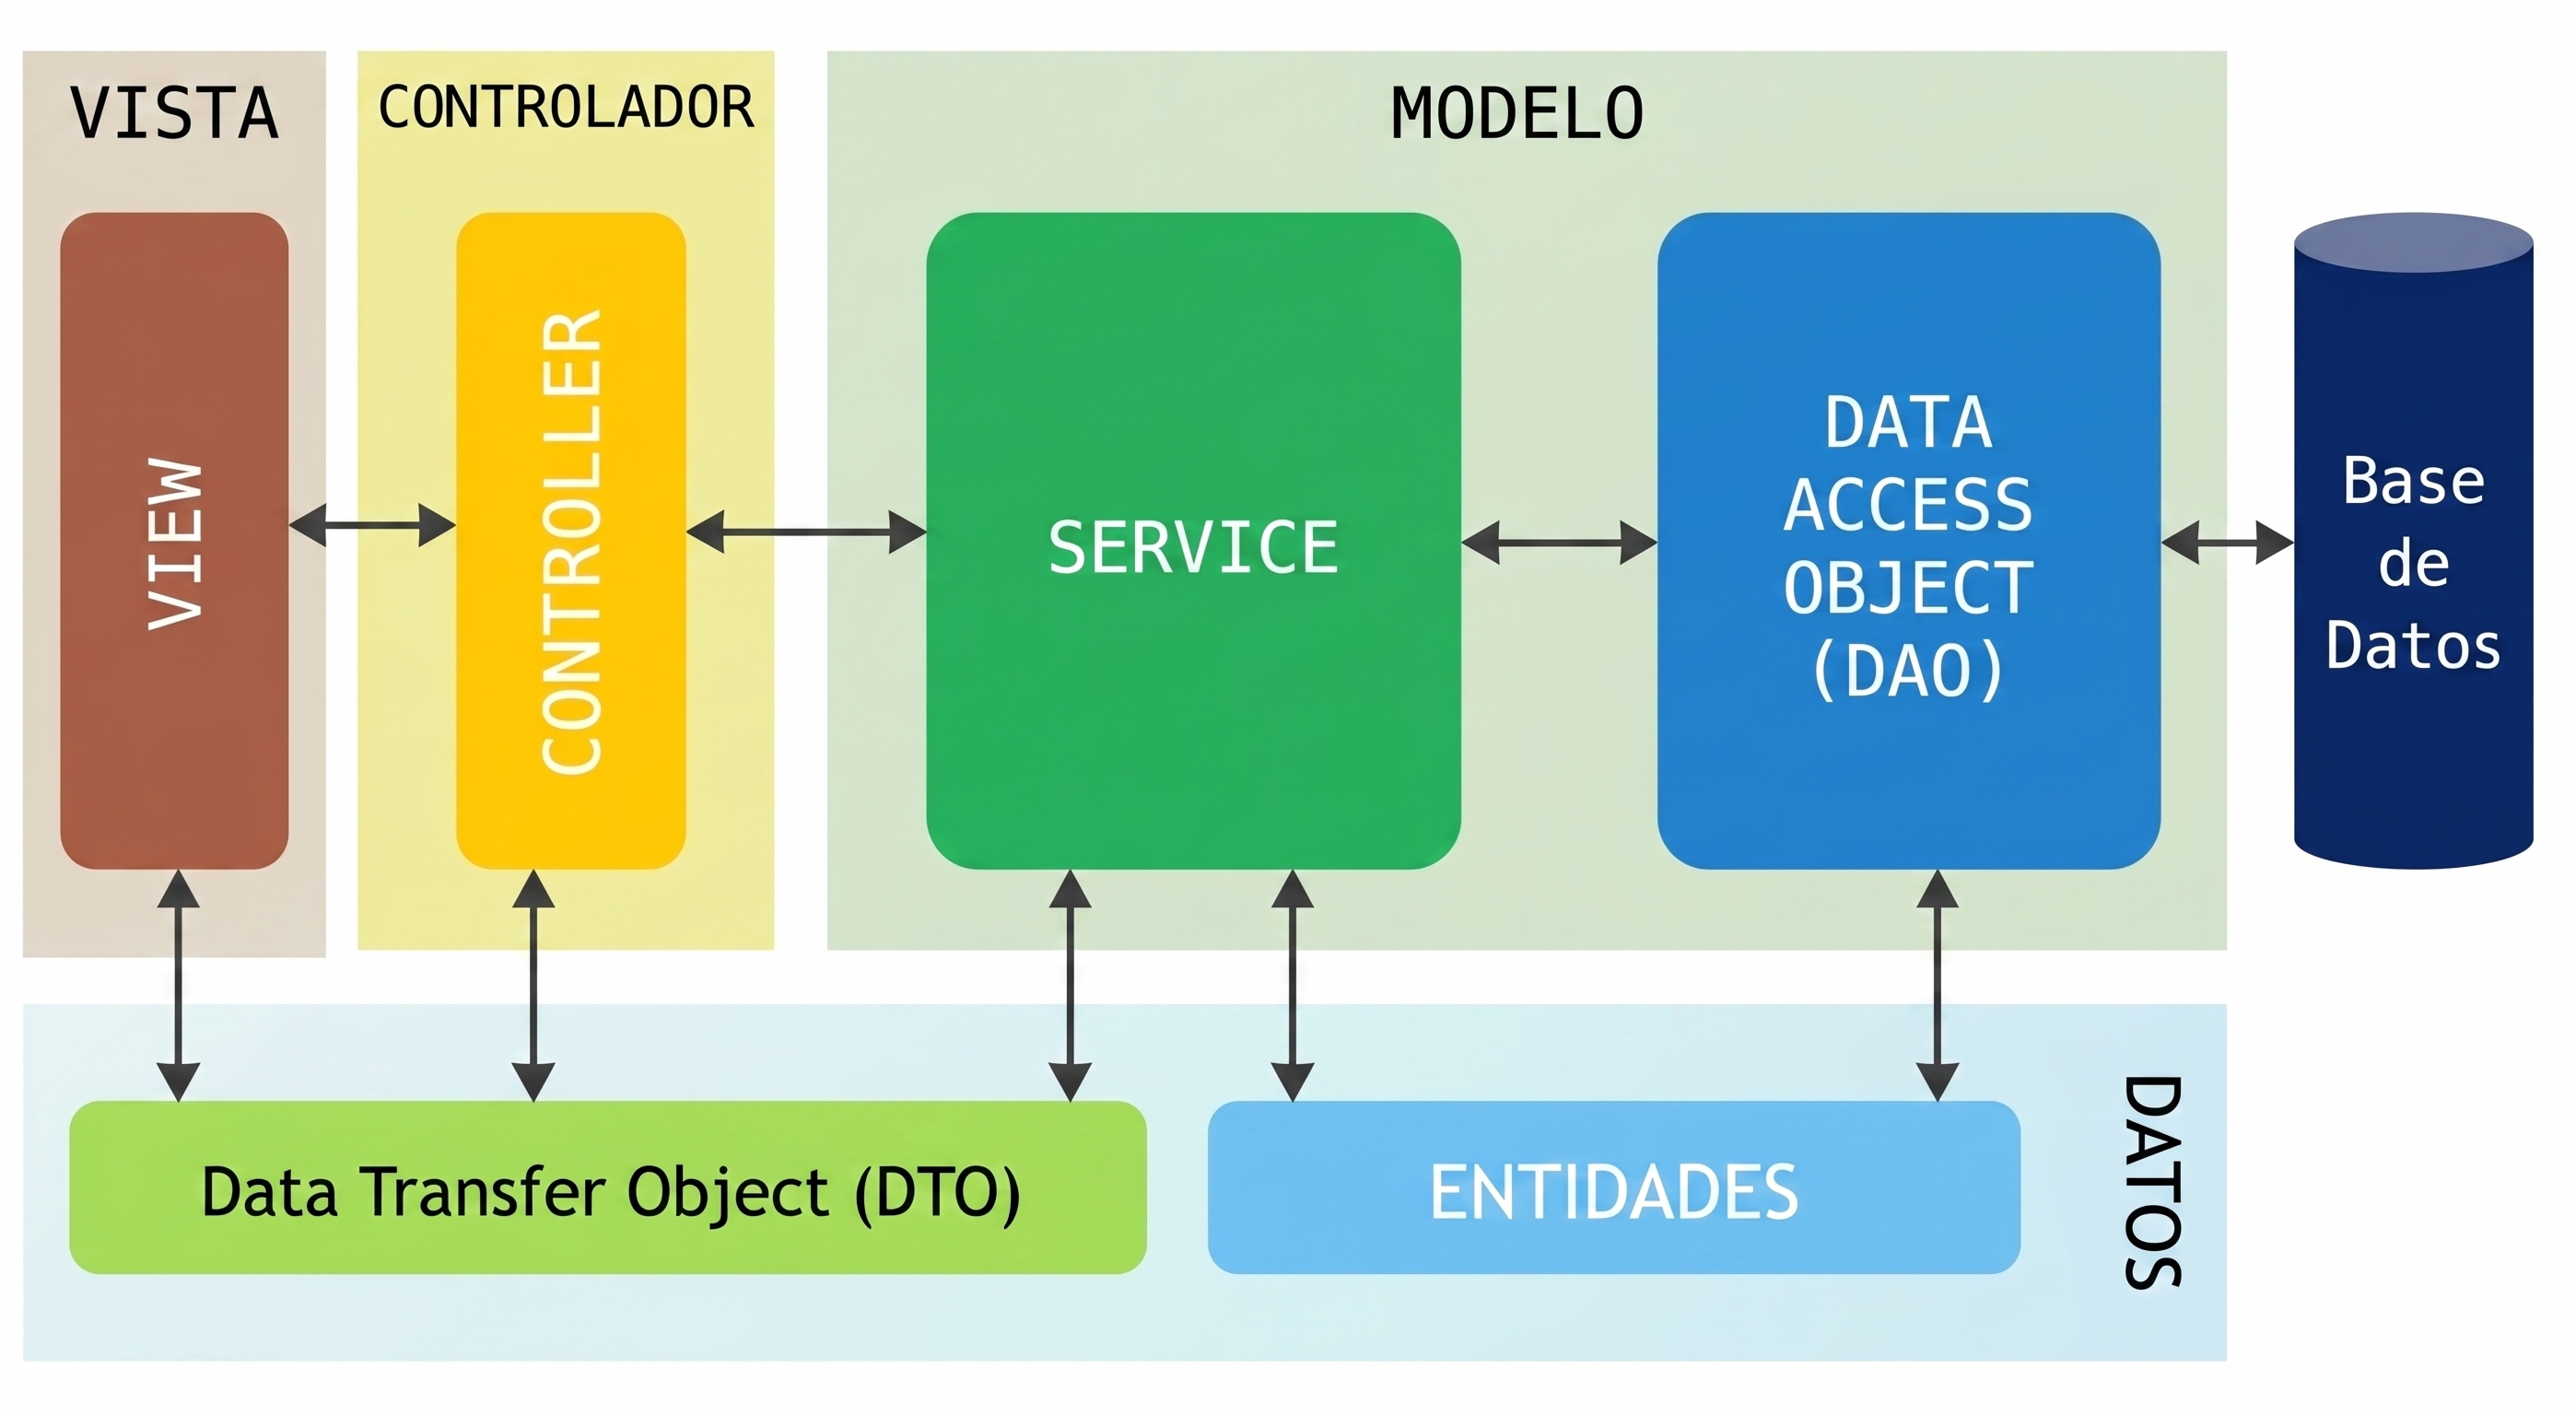
\includegraphics[width=0.80\linewidth]{assets/mermeid/PatronMVC.png}}{\textit{Fuente: Patrones de diseño DTO y Service, Eduardo Guzmán De los Riscos (guzman@lcc.uma.es)}}
\end{figure}
\par
\vspace{5mm}
La comunicación entre frontend y backend se realiza
exclusivamente mediante una API REST sobre HTTPS, autenticada con JWT. % chktex 13
El navegador del usuario nunca accede directamente a la base de datos: todas las
reglas de negocio, validaciones y comprobaciones de autorización residen en el
backend, lo que mantiene un perímetro de confianza claro y simplifica las
auditorías de seguridad.    
\begin{figure}[H]
    \centering
    \caption{Diagrama de arquitectura API RESTful}
    \copyrightbox[b]{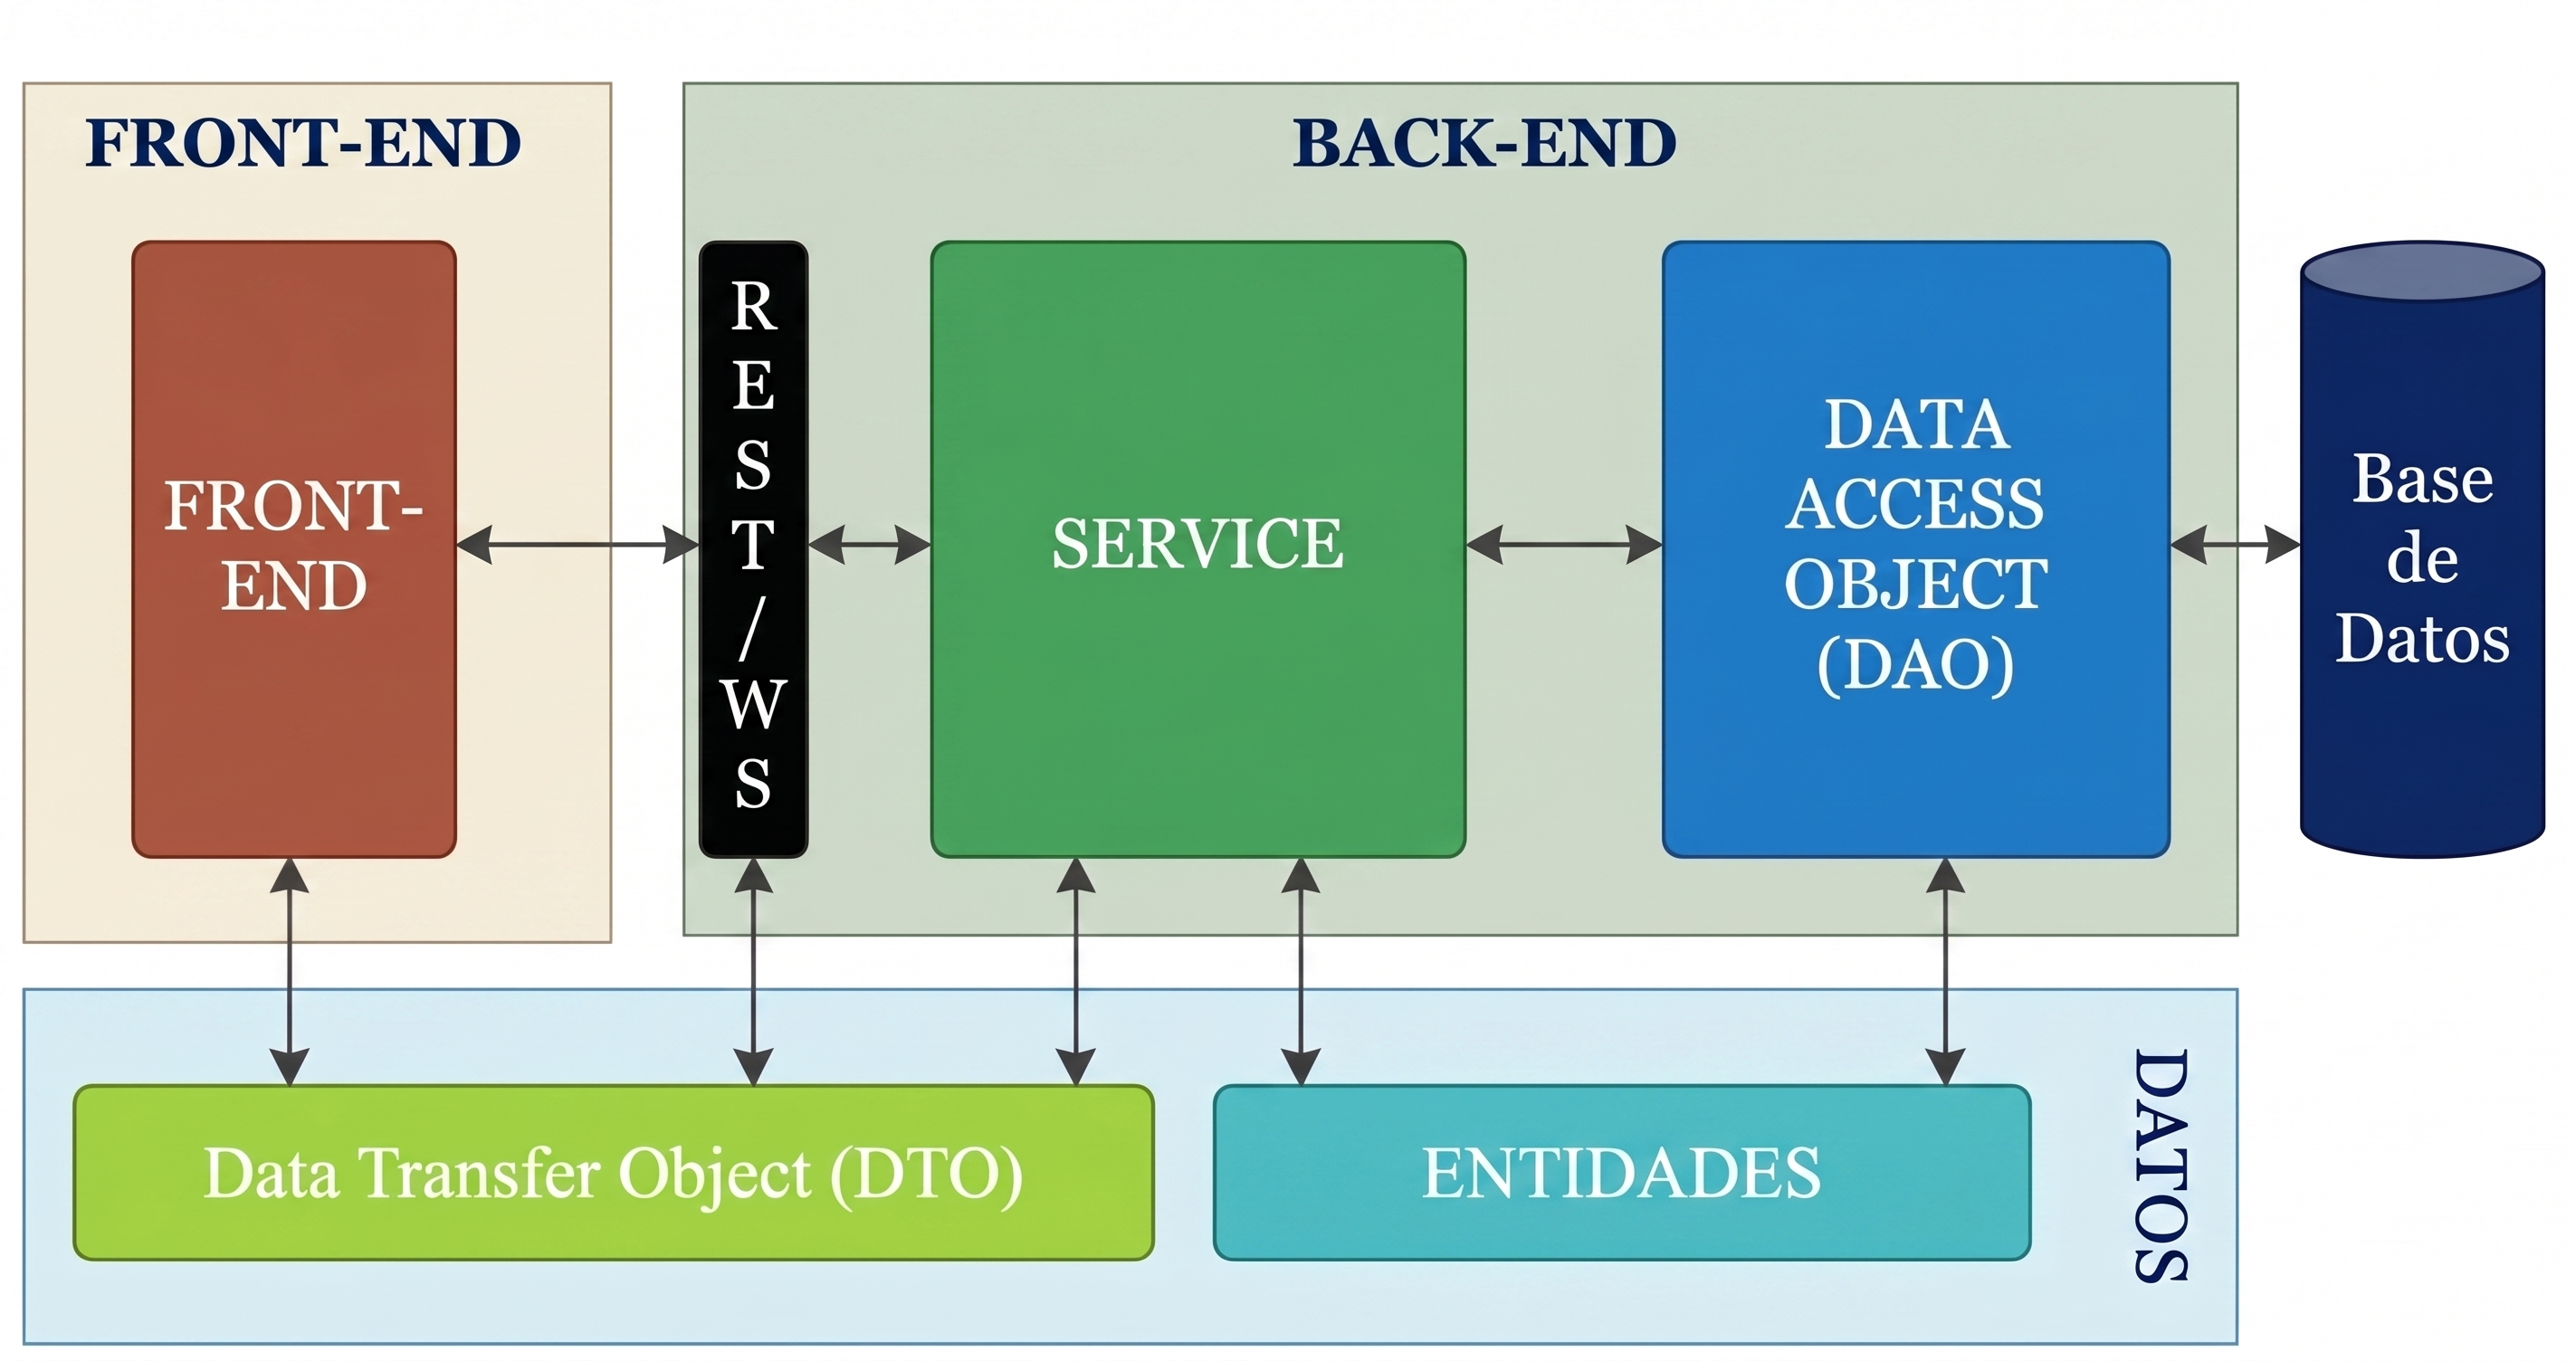
\includegraphics[width=0.80\linewidth]{assets/mermeid/ArquitecturaGeneral.png}}{\textit{Fuente: Patrones de diseño DTO y Service, Eduardo Guzmán De los Riscos (guzman@lcc.uma.es)}}
\end{figure}
\par
\vspace{5mm}
El conjunto se empaqueta mediante \textbf{Docker} y se despliega en \textbf{Render}, que
proporciona la infraestructura en la nube, el balanceo de carga, el
certificado TLS y la conexión privada entre el servicio web y la base de datos.
La gestoría fiscal externa, las entidades financiadoras y las autoridades
sanitarias son actores externos al sistema: interactúan con él de forma
indirecta, recibiendo informes exportados (CSV, PDF, JSON) generados desde la
aplicación.
\begin{figure}[H]
    \centering
    \caption{Diagrama de arquitectura general y fronteras del sistema}
    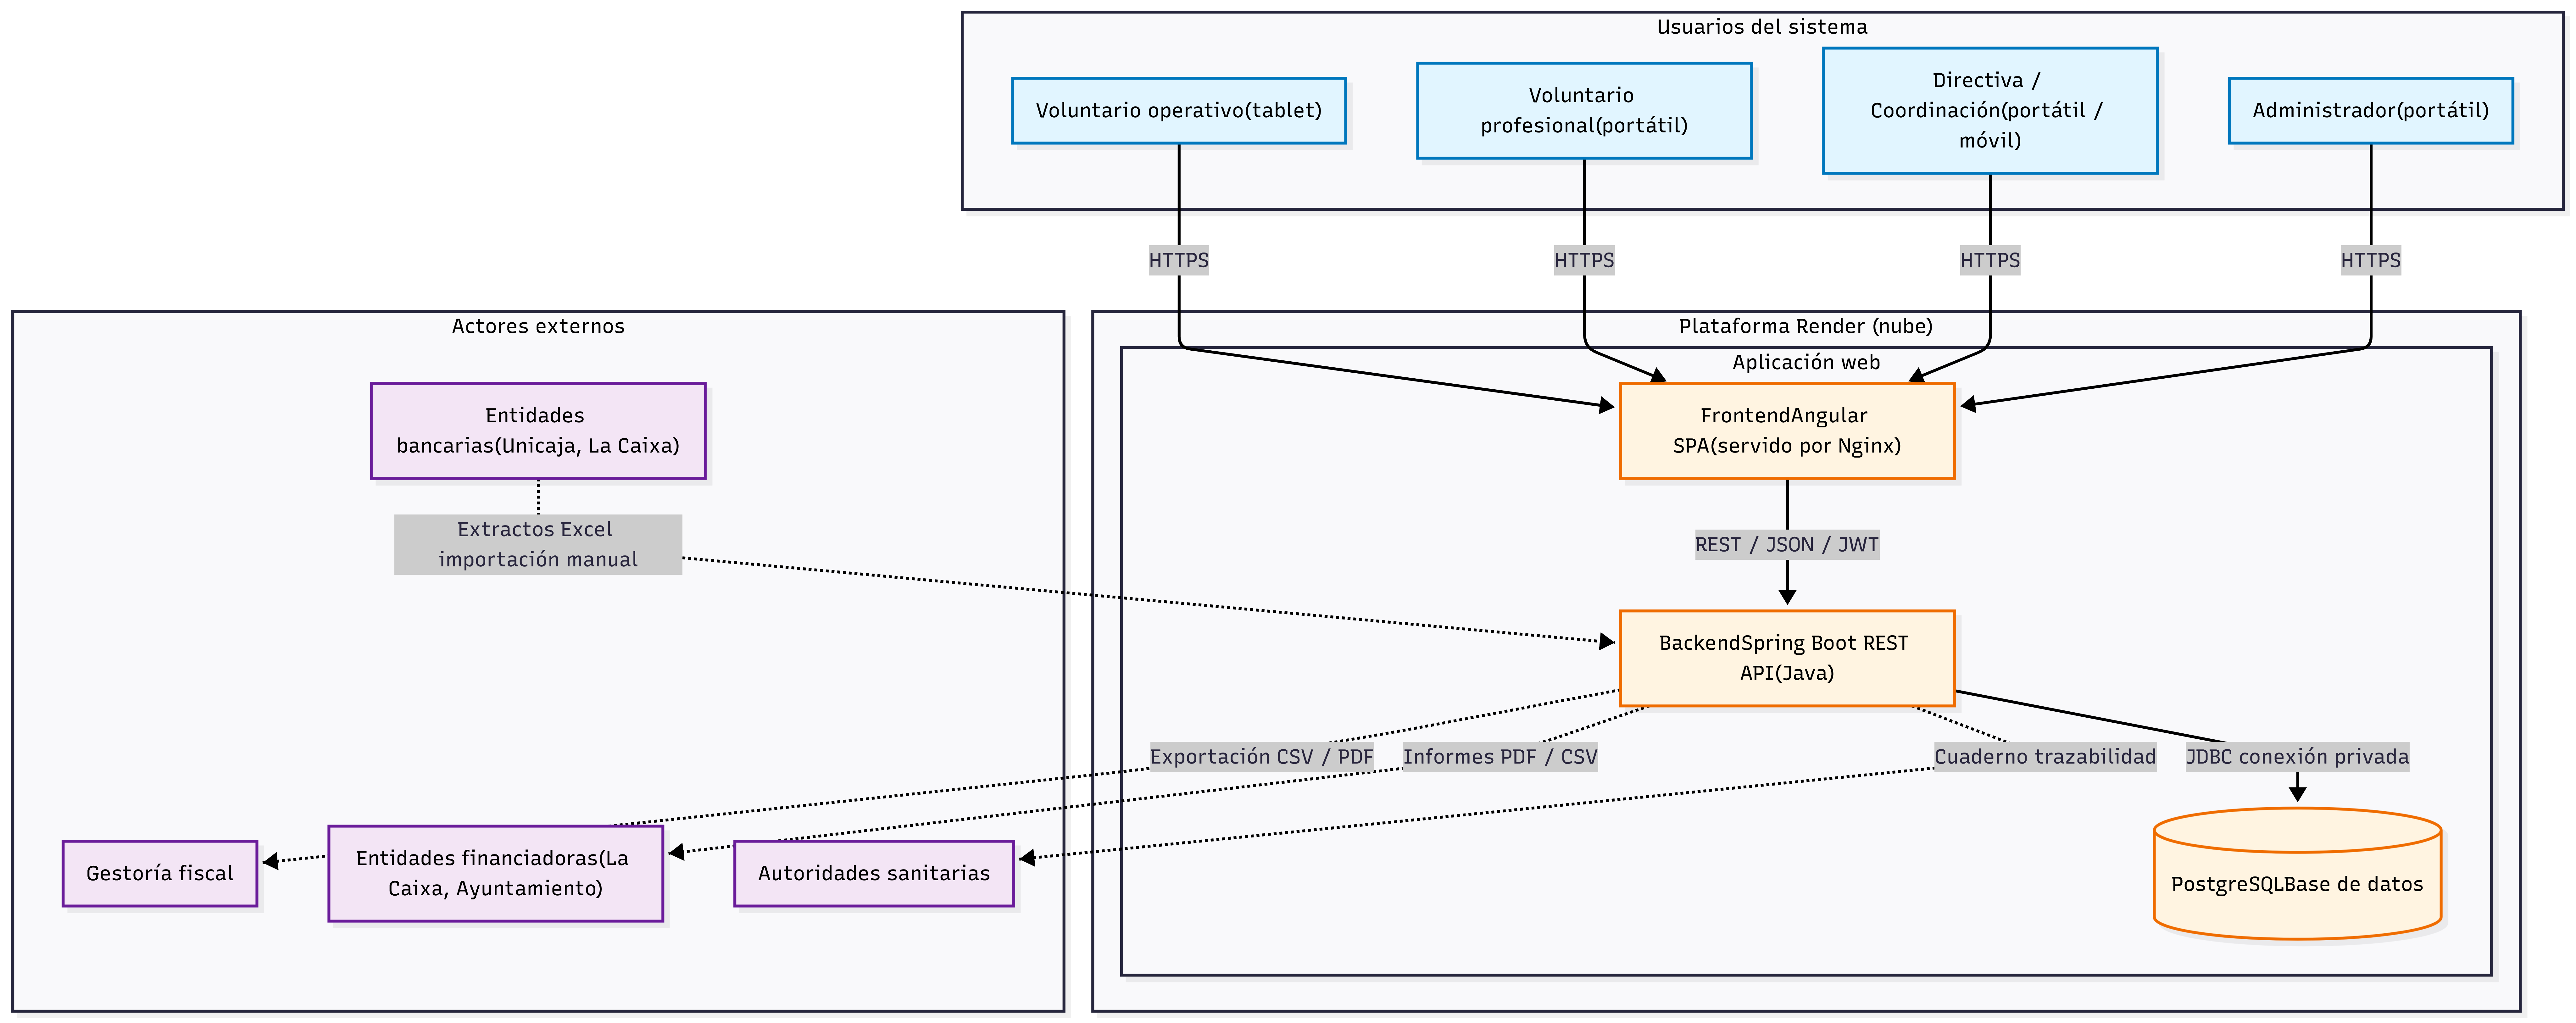
\includegraphics[width=1\linewidth]{assets/mermeid/Arquitectura-Fronteras-delSistema.png}
\end{figure}
\par
\vspace{5mm}
Las flechas de trazo continuo representan interacción en tiempo real mediada
por el sistema; las de trazo discontinuo representan flujos diferidos de
intercambio de información (importaciones manuales de extractos bancarios,
generación periódica de informes para terceros).


\subsection{Funciones del Producto}\hypertarget{section2.2}{anchor text}
A continuación se resume el alcance de cada una de las áreas funcionales en el sistema a un nivel 
suficiente para entender su propósito sin entrar en el detalle de cada operación.
\begin{itemize}
    \item \textbf{Gestión de cuentas y autenticación}. Permite crear, modificar y dar de baja
    cuentas de voluntario en el sistema, así como gestionar el inicio y cierre de
    sesión, la recuperación de contraseña y la protección frente a accesos no
    autorizados. Es la puerta de entrada al sistema: ninguna otra función está
    disponible sin haber atravesado este bloque.

    \item \textbf{Control de acceso y roles}. Implementa el sistema de permisos: define qué
    roles existen (administrador, operativo, profesional, puente, agente externo
    temporal), qué nivel de seguridad tiene cada voluntario para visualizar datos
    sensibles (\texttt{BÁSICO} o \texttt{PRIVILEGIADO}) y qué funciones específicas puede ejecutar
    cada uno (entregar ropa, agendar servicio, registrar gastos, leer notas
    psicológicas, importar extractos bancarios, etc.). Incluye el mecanismo de
    habilitación temporal que permite a la coordinación abrir puntualmente el
    acceso a un voluntario profesional sobre el expediente de un amigo concreto.

    \item \textbf{Gestión del amigo.} Mantiene el expediente de cada persona atendida con un
    modelo de \textbf{ficha progresiva} que escala según el nivel de confianza
    alcanzado: en el primer contacto sólo se registra el nombre; con la
    recurrencia se añaden alias, tallas y datos básicos; sólo tras una entrevista
    de profundidad se incorpora el DNI y los datos sensibles. Cada amigo dispone
    de un histórico completo.

    \item \textbf{Servicios y agendamiento.} Gestiona el catálogo de servicios que el centro
    ofrece: duchas, asistencia jurídica, médica, psicológica, podología,
    extranjería, educativa, entre otras y permite agendarlos con fecha, hora y voluntario
    asignado. Implementa control de capacidad por turno (por ejemplo, máximo
    cuatro duchas por turno para evitar cuellos de botella) y la regla de
    pre-requisito: sin agendamiento no se presta el servicio.

    \item \textbf{Inventario, entregas y lavandería.} El \textbf{armario general} opera como un stock
    impersonal: se registran las donaciones recibidas, se controla el inventario
    por tipo y talla, y cada entrega a un amigo decrementa automáticamente el
    stock aplicando reglas de frecuencia configurables (por ejemplo, un par de
    zapatillas cada tres meses para el mismo amigo). No se opera de forma personal: el centro no recibe ropa 
    propia del amigo, la lava y se la devuelve a la misma persona; se va rotando la ropa a necesidad del amigo que la solicite.

    \item \textbf{Trazabilidad alimentaria.} Implementa el cuaderno de entradas y salidas
    exigido por la Ley 1/2025. Registra el origen de cada alimento (compra
    propia, donación de entidad con convenio, donación particular, etc.), su lote y
    fecha de caducidad, su clasificación según prioridad legal de
    aprovechamiento, las verificaciones de higiene del producto y del lugar de
    almacenamiento, y la temperatura de salida en el caso de productos
    refrigerados. Asocia tickets, albaranes y convenios (cuando existen), y permite
    generar el cuaderno completo en formato apto para inspección sanitaria.

    \item \textbf{Gestión contable.} Reproduce y automatiza el flujo que la contabilidad 
    que se lleva hoy manualmente en Excel. Mantiene un plan de cuentas
    parametrizable (por ejemplo, códigos como 600 para gastos de comunidad, 5720 para bancos,
    6260 para servicios bancarios\ldots), permite importar los extractos bancarios en formato Excel, 
    y aplica reglas de mapeo automático que
    asocian conceptos recurrentes a las cuentas correspondientes, generando los asientos de diario sin intervención
    manual. 
    \par
    Diferencia los flujos de \textbf{tarjeta bancaria} y \textbf{caja chica} en
    efectivo, categoriza cada gasto como propio de la Casa, del amigo o mixto, y
    permite vincularlo opcionalmente a un amigo o a un servicio concreto para
    obtener trazabilidad por persona (esto ayuda a responder preguntas del tipo \textit{``¿cuánto hemos gastado en Francisco este
    semestre?''}). % chktex 38

    \item \textbf{Reportes, informes y visualización.} Centraliza la salida de datos del
    sistema. Ofrece un panel visual con los indicadores que la directiva consulta
    con mayor frecuencia (gastos por categoría, número de servicios prestados al
    mes, costes de alimentación, número de cafés servidos), genera informes
    numéricos exactos por mes, semestre o año para
    presentar a entidades financiadoras, y permite exportar la información en
    PDF, CSV y JSON. Soporta filtros y consultas \textit{ad-hoc}\footnote{Una \textit{consulta ad-hoc} (del latín ``para esto'') es una búsqueda o informe de datos creado desde cero para responder a una pregunta puntual e inmediata.} por amigo, servicio, % chktex 13
    periodo, voluntario o cuenta contable.

    \item \textbf{Puente analógico-digital y carga inicial.} Reconoce que una parte
    significativa del voluntariado opera con papel y debe seguir pudiendo
    hacerlo. El sistema prepara planillas con exactamente los mismos campos que
    las entidades de la base de datos, de modo que un voluntario
    analógico rellena a mano y otro voluntario carga después esos datos al
    sistema. Adicionalmente, soporta la importación masiva de los datos
    históricos contenidos hoy en las hojas Excel de la coordinación y la
    contabilidad, validando duplicados y errores de formato durante la carga.
\end{itemize}
\par
\vspace{5mm}

\begin{figure}[H]
    \centering
    \caption{Organización funcional del sistema}
    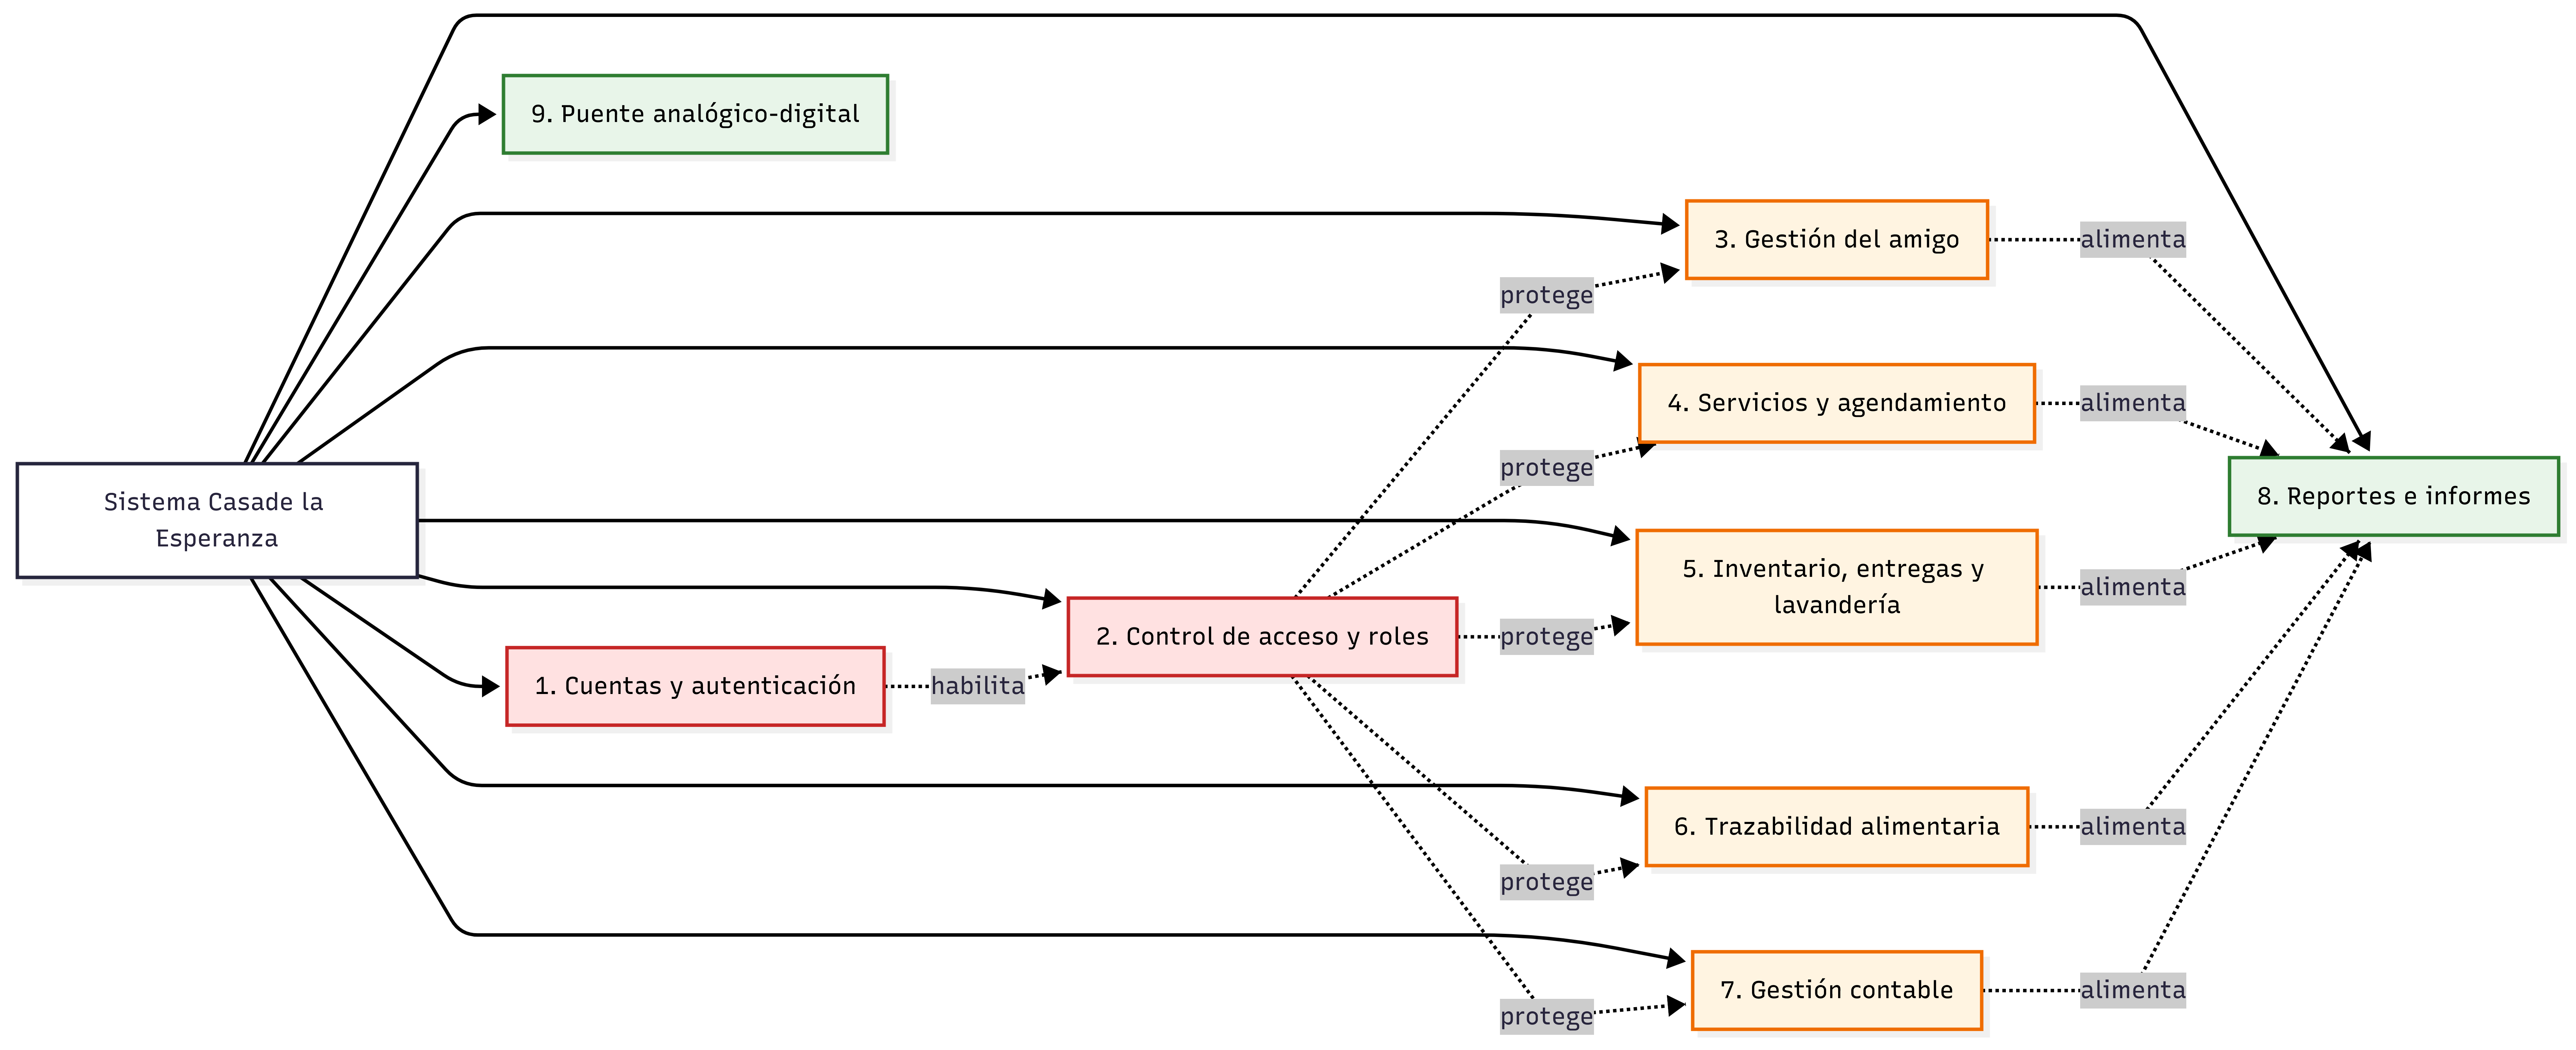
\includegraphics[width=1\linewidth]{assets/mermeid/organizacionFuncional.png}
\end{figure}
\par
\vspace{5mm}

\subsection{Requisitos Futuros}\label{section_RequisitosFuturos}
Esta sección propone mejoras y extensiones del sistema que no forman parte del
alcance de la versión inicial pero que se han identificado durante el proceso
de captura de requisitos como deseables a medio o largo plazo.

\begin{itemize}
    \item \textbf{Sistema de notificaciones automáticas.} Envío proactivo de avisos a
    voluntarios y miembros de la directiva ante eventos relevantes: alimentos
    próximos a caducar, stock de armario por debajo de umbral, citas profesionales
    del día siguiente, gastos pendientes de aprobación, fin de vigencia de un
    convenio de donación. Los canales contemplados son correo electrónico y
    WhatsApp.

    \item \textbf{Trazabilidad de comunicaciones externas extendida.} Aunque el registro
    manual de comunicaciones vinculadas al amigo (correos a policía,
    ayuntamiento, citas externas) está contemplado como funcionalidad de la
    versión inicial (ver \hyperlink{RF3.6}{RF3.6}), la integración automática con la % chktex 2
    bandeja de correo de modo que los correos enviados o
    recibidos relacionados con un amigo se asocien automáticamente a su perfil,
    con análisis de remitente, destinatario y palabras clave se considera una
    mejora futura.

    \item \textbf{Diseño responsive multi-dispositivo.} La versión actual del proyecto esta destinada a ser una aplicación web 
    principalmente accesible y operable desde un ordenador. Diseño responsive para acomodar dispositivos de distintas dimensiones 
    como tablets o móviles es una solicitud real, pero fuera del alcance inicial.

    \item \textbf{Migración de la base de datos.} Si el
    volumen de datos crece significativamente (por ejemplo, si la asociación
    amplía su radio de acción o si se incorporan otras delegaciones), puede
    ser necesario migrar de la instancia PostgreSQL gestionada por Render a
    una solución de mayor capacidad, replicación geográfica o particionado.

    \item \textbf{Internacionalización.} La versión inicial está disponible únicamente en
    español (España). La incorporación de inglés (US/UK) facilitaría la
    interacción con voluntarios y amigos no hispanohablantes en la propia
    interfaz, especialmente en los formularios que se cumplimentan junto al
    amigo.

    \item \textbf{RF6.x Gestión de convenios con entidades donantes} \\
    El sistema debe permitir registrar y mantener los convenios de donación
    firmados con entidades aportantes regulares (Mercadona, Bancosol, etc.).
    \begin{description}
        \item[-] El sistema avisa visualmente cuando un convenio se aproxima a su
        fecha de vencimiento (por defecto, 30 días antes).
    \end{description}
    \par
    Este requisito formaba parte del DGR DOC001 pero cuando se revisó con el cliente, a pesar que la Ley 1/2025 exige 
    en el articulo 6.4.b) que los agentes de la cadena alimentaria (como Mercadona) promuevan convenios para donar sus excedentes de alimentos a  % chktex 10 
    asociaciones como la Casa de la Esperanza, se decidió dejar fuera ya que no está en su interés tener esta clase de convenios por el momento.
\end{itemize} % chktex 17